\documentclass[11pt,a4paper]{article}

\usepackage[margin=1.5cm]{geometry}
\usepackage{graphicx}
\usepackage{listings}
\usepackage{xcolor}
\usepackage{hyperref}
\usepackage{tikz}

% Hyperlink styling
\hypersetup{
    colorlinks=true,
    linkcolor=blue,
    filecolor=magenta,      
    urlcolor=blue,
    pdftitle={Computer Graphics Lab 2 Report},
    pdfauthor={Shahriar Alom Masud}
}

% Python syntax highlighting configuration
\definecolor{codegreen}{rgb}{0,0.6,0}
\definecolor{codegray}{rgb}{0.5,0.5,0.5}
\definecolor{codepurple}{rgb}{0.58,0,0.82}
\definecolor{backcolour}{rgb}{0.97,0.97,0.97}

\lstdefinestyle{pythonstyle}{
    backgroundcolor=\color{backcolour},   
    commentstyle=\color{codegreen}\itshape,
    keywordstyle=\color{blue}\bfseries,
    numberstyle=\tiny\color{codegray},
    stringstyle=\color{codepurple},
    basicstyle=\ttfamily\scriptsize,
    breaklines=true,                 
    numbers=left,                    
    numbersep=4pt,                  
    tabsize=4,
    frame=single,
    rulecolor=\color{lightgray}
}

\lstset{style=pythonstyle}

\begin{document}

% ==============================================================================
% COVER PAGE (Matches University Standard Format)
% ==============================================================================
\begin{titlepage}
    % Page Border using TikZ
    \begin{tikzpicture}[remember picture, overlay]
        \draw[line width=1.2pt] 
            ([shift={(1.2cm,-1.2cm)}]current page.north west) 
            rectangle 
            ([shift={(-1.2cm,1.2cm)}]current page.south east);
        \draw[line width=0.5pt] 
            ([shift={(1.32cm,-1.32cm)}]current page.north west) 
            rectangle 
            ([shift={(-1.32cm,1.32cm)}]current page.south east);
    \end{tikzpicture}

    \centering
    \vspace*{0.5cm}

    % Header Title
    {\large \textbf{COMPUTER GRAPHICS LAB REPORT}}\\[0.25cm]
    {\normalsize \textbf{LAB 02: BASIC 2D DRAWING WITH TURTLE GRAPHICS}}\\[0.45cm]

    \noindent\rule{0.88\textwidth}{0.85pt}\\[0.55cm]

    {\normalsize \textbf{COURSE CODE: IRE 404}}\\[0.18cm]
    {\normalsize \textbf{COURSE TITLE: COMPUTER GRAPHICS AND ANIMATION SESSIONAL}}\\[1.5cm]

    % Student Info
    {\small \textit{SUBMITTED BY -}}\\[0.28cm]
    {\normalsize \textbf{SHAHRIAR ALOM MASUD}}\\[0.15cm]
    {\footnotesize STUDENT ID: 2201032}\\[0.1cm]
    {\footnotesize SESSION: 2022--2023}\\[1.2cm]

    % Instructor Info
    {\small \textit{SUBMITTED TO -}}\\[0.28cm]
    {\normalsize \textbf{FARZANA AKTER}}\\[0.15cm]
    {\footnotesize ASSISTANT PROFESSOR}\\[0.1cm]
    {\footnotesize DEPARTMENT OF IRE, UFTB}\\[1.2cm]

    % University Logo
    
\includegraphics[width=2.5cm]{screenshots/uftb_logo.png}\\[1.3cm]

    % University & Faculty Details
    \vfill
    {\footnotesize FACULTY OF CYBER PHYSICAL SYSTEM ENGINEERING}\\[0.18cm]
    {\footnotesize DEPARTMENT OF INTERNET OF THINGS AND ROBOTICS ENGINEERING (IRE)}\\[0.18cm]
    {\footnotesize UNIVERSITY OF FRONTIER TECHNOLOGY, BANGLADESH}\\[0.45cm]
    {\footnotesize OCTOBER 12, 2026}
    \vspace*{0.3cm}
\end{titlepage}

\newpage
\pagenumbering{arabic}

% ==============================================================================
% TASK 1: SMILING FACE
% ==============================================================================
\section*{Task 1: Drawing a Smiling Face}
\noindent\rule{\textwidth}{0.6pt}\vspace{0.15cm}

\noindent\textbf{GitHub Repository Link:}\\
\href{https://github.com/Masud744/Computer-Graphics-Lab/blob/main/task1.py}{\texttt{https://github.com/Masud744/Computer-Graphics-Lab/blob/main/task1.py}}\vspace{0.25cm}

\noindent
\begin{minipage}[t]{0.56\textwidth}
\textbf{Python Source Code (\texttt{task1.py}):}
\vspace{0.1cm}
\lstinputlisting[language=Python]{../task1.py}
\end{minipage}
\hfill
\begin{minipage}[t]{0.41\textwidth}
\textbf{Problem Description:}
\vspace{0.1cm}
{\footnotesize Draw a face enclosed in a black circle (radius 300), small green blots for eyes, a thick blue triangle for a nose, and a red smiling mouth. The smiling mouth is formed by drawing a red blot, and then drawing a white blot slightly higher to leave a crescent of red.}

\vspace{0.4cm}
\textbf{Output Visualization:}
\vspace{0.1cm}
\begin{center}
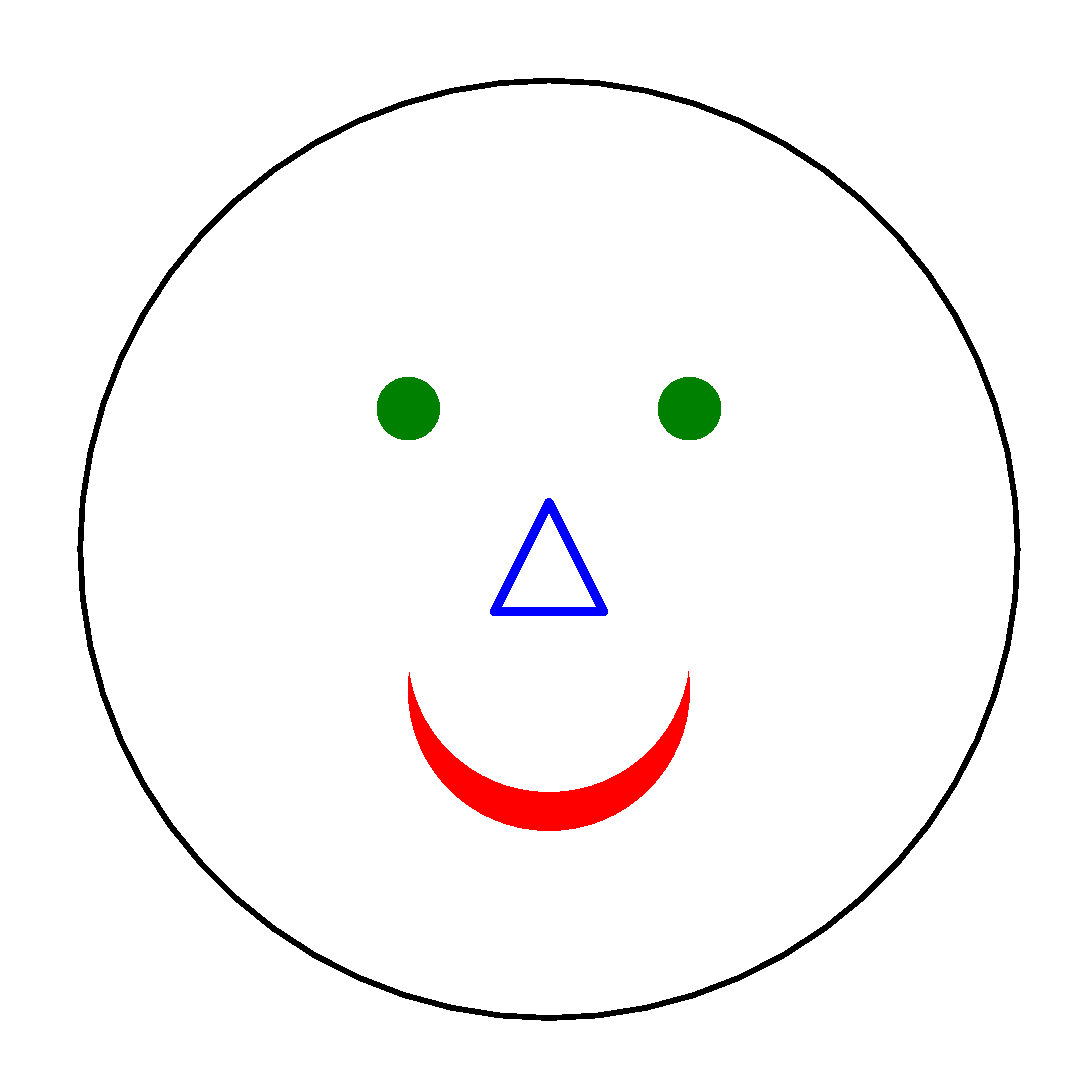
\includegraphics[width=0.92\textwidth]{screenshots/task1_output.png}
\end{center}

\vspace{0.2cm}
\textbf{Observation:}
\vspace{0.1cm}
{\footnotesize The mouth must be drawn before the nose and eyes. Because the white blot creates the crescent smile by partially covering the underlying shape, drawing the mouth afterward would overwrite parts of the nose with white.}
\end{minipage}

\newpage

% ==============================================================================
% TASK 2: FLAG (10:6)
% ==============================================================================
\section*{Task 2: Flag Rectangle and Proportions (10:6)}
\noindent\rule{\textwidth}{0.6pt}\vspace{0.15cm}

\noindent\textbf{GitHub Repository Link:}\\
\href{https://github.com/Masud744/Computer-Graphics-Lab/blob/main/task2.py}{\texttt{https://github.com/Masud744/Computer-Graphics-Lab/blob/main/task2.py}}\vspace{0.25cm}

\noindent
\begin{minipage}[t]{0.56\textwidth}
\textbf{Python Source Code (\texttt{task2.py}):}
\vspace{0.1cm}
\lstinputlisting[language=Python]{../task2.py}
\end{minipage}
\hfill
\begin{minipage}[t]{0.41\textwidth}
\textbf{Problem Description:}
\vspace{0.1cm}
{\footnotesize Draw a green background rectangle with proportions of approximately 10:6 (length). Draw a red circle inside the rectangle. Fill the rectangle with green and the circle with red. Position the centre of the red circle at one-fifth ($1/5$) of the rectangle's length from the left edge.}

\vspace{0.4cm}
\textbf{Output Visualization:}
\vspace{0.1cm}
\begin{center}

\includegraphics[width=0.95\textwidth]{screenshots/task2_output.png}
\end{center}

\vspace{0.2cm}
\textbf{Observation:}
\vspace{0.1cm}
{\footnotesize In the authentic National Flag of Bangladesh, the centre of the red circle is located at $9/20$ ($45\%$) of the length from the left edge. In this lab task, placing the circle at $1/5$ ($20\%$) from the left edge visibly shifts the circle to the far-left border, as observed.}
\end{minipage}

\newpage

% ==============================================================================
% TASK 3: OVERLAPPING SQUARES
% ==============================================================================
\section*{Task 3: Overlapping Concentric Squares (8-Point Star)}
\noindent\rule{\textwidth}{0.6pt}\vspace{0.15cm}

\noindent\textbf{GitHub Repository Link:}\\
\href{https://github.com/Masud744/Computer-Graphics-Lab/blob/main/task3.py}{\texttt{https://github.com/Masud744/Computer-Graphics-Lab/blob/main/task3.py}}\vspace{0.25cm}

\noindent
\begin{minipage}[t]{0.56\textwidth}
\textbf{Python Source Code (\texttt{task3.py}):}
\vspace{0.1cm}
\lstinputlisting[language=Python]{../task3.py}
\end{minipage}
\hfill
\begin{minipage}[t]{0.41\textwidth}
\textbf{Problem Description:}
\vspace{0.1cm}
{\footnotesize Draw the shape consisting of two overlapping squares sharing the identical center point. One square is aligned horizontally/vertically ($0^\circ$), and the second square is rotated by $45^\circ$, forming an 8-pointed star shape.}

\vspace{0.4cm}
\textbf{Output Visualization:}
\vspace{0.1cm}
\begin{center}
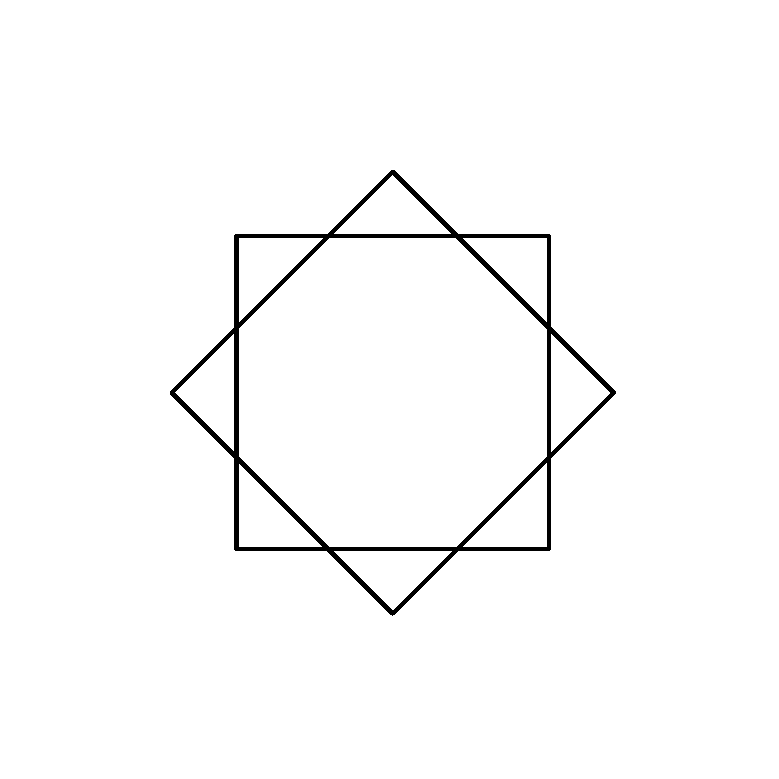
\includegraphics[width=0.85\textwidth]{screenshots/task3_output.png}
\end{center}

\vspace{0.2cm}
\textbf{Observation:}
\vspace{0.1cm}
{\footnotesize Both squares have equal side length $S = 200$ and center at $(0, 0)$. The straight square is drawn from corner $(-S/2, -S/2)$. The $45^\circ$ rotated square is drawn with corner offset $R = \frac{S}{\sqrt{2}} \approx 141.4$ along the vertical axis, forming an 8-pointed star.}
\end{minipage}

\newpage

% ==============================================================================
% TASK 4: ELEGANT ROTATED SQUARES
% ==============================================================================
\section*{Task 4: Elegant Rotated Squares Pattern}
\noindent\rule{\textwidth}{0.6pt}\vspace{0.15cm}

\noindent\textbf{GitHub Repository Link:}\\
\href{https://github.com/Masud744/Computer-Graphics-Lab/blob/main/task4.py}{\texttt{https://github.com/Masud744/Computer-Graphics-Lab/blob/main/task4.py}}\vspace{0.25cm}

\noindent
\begin{minipage}[t]{0.56\textwidth}
\textbf{Python Source Code (\texttt{task4.py}):}
\vspace{0.1cm}
\lstinputlisting[language=Python]{../task4.py}
\end{minipage}
\hfill
\begin{minipage}[t]{0.41\textwidth}
\textbf{Problem Description:}
\vspace{0.1cm}
{\footnotesize Draw the 5-square rotational pattern. Think carefully about how you might be able to draw this elegantly (efficiently and readably).}

\vspace{0.4cm}
\textbf{Output Visualization:}
\vspace{0.1cm}
\begin{center}
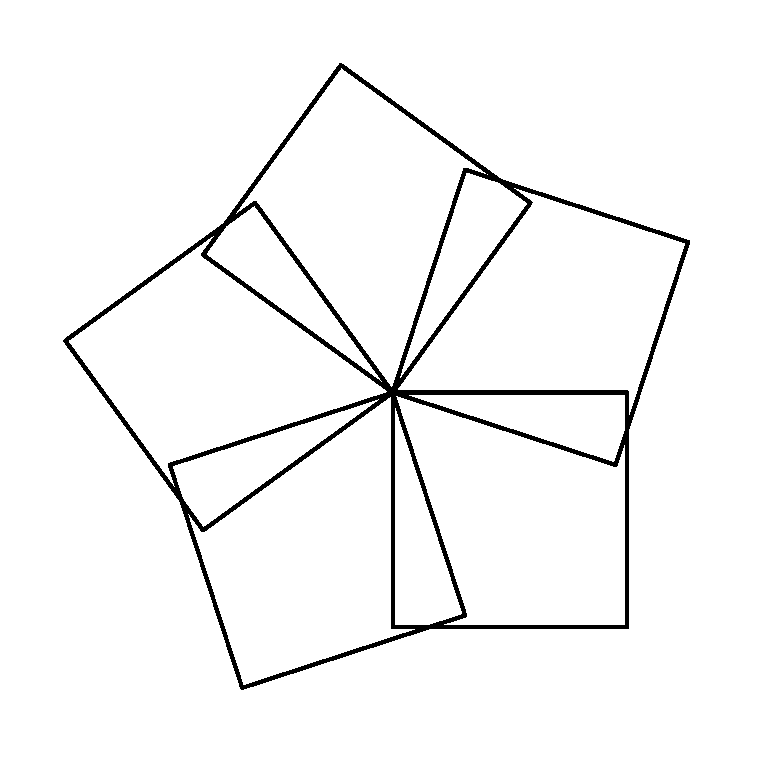
\includegraphics[width=0.85\textwidth]{screenshots/task4_output.png}
\end{center}

\vspace{0.2cm}
\textbf{Observation:}
\vspace{0.1cm}
{\footnotesize The pattern exhibits 5-fold rotational symmetry about a common corner vertex. Instead of repetitive code, it is implemented using a concise nested loop: repeating 5 times, turning right by $360^\circ / 5 = 72^\circ$ after each 4-sided square with $90^\circ$ turns.}
\end{minipage}

\end{document}
